\documentclass[a4paper,12pt]{article}
\usepackage{geometry}
\geometry{left=2.5cm,right=2.5cm,top=2.8cm,bottom=2.8cm}
\usepackage{amsmath,amssymb}
\usepackage{physics}
\usepackage{ctex}
\usepackage{graphicx}
\usepackage{float}
\usepackage{subcaption}
\usepackage{booktabs}
\usepackage{listings}
\usepackage{xcolor}


\lstset{
    language=Matlab,
    basicstyle=\ttfamily\small,
    keywordstyle=\color{blue}\bfseries,
    commentstyle=\color{green!40!black}\itshape,
    stringstyle=\color{red!70!black},
    numbers=left,
    numberstyle=\tiny\color{gray},
    frame=single,
    breaklines=true,
    showstringspaces=false,
    captionpos=b
}

\usepackage{fancyhdr}
\pagestyle{fancy}
\fancyhf{}
\fancyhead[L]{Numerical Study of Near BH Spacetimes}
\fancyhead[R]{Tang Yi \& Zhou Jingzi}
\fancyfoot[C]{\thepage}

\title{\bfseries
GR背景下的时空行为的数值模拟研究\\[0.3em]
\large 从Schwarzschild到RN黑洞}
\author{
学生 \& 同学\\
\small 北京师范大学\ 物理与天文学院\\
\small 学号：[学号已脱敏] \& [学号已脱敏]
}
\date{\small \today}
\begin{document}

\maketitle

\thispagestyle{empty}

\begin{abstract}
本文在广义相对论框架下，面向静态球对称黑洞时空构建了一套可复用的数值模拟与可视化流程，重点比较史瓦西（Schwarzschild）解与赖斯纳--诺德斯特洛姆（Reissner--Nordström, RN）带电黑洞解在因果结构、测地线动力学与光学成像方面的差异。我们实现并串联了若干相互独立的计算模块：彭罗斯图（Penrose diagram）的保角压缩绘制、类时测地线在内视界附近的数值积分、测试粒子轨道进动的有效势分析与轨迹模拟，以及基于逆向光线追踪（backward ray tracing）的黑洞吸积盘成像渲染。数值结果直观展示了RN时空的双视界结构（$r_\pm$）、内视界附近的因果性质变化，以及电荷参数 $Q/M$ 改变对阴影大小与引力透镜特征的影响；特别地，当 $Q/M>1$ 时事件视界消失，对应裸奇点情形，其成像呈现出与常规黑洞显著不同的中心高亮与透镜结构。本文的模拟结果与解析预言一致，为强场区广义相对论的教学与数值实验提供了可视化支撑。
\end{abstract}

\newpage
\tableofcontents
\newpage

\section{引言与理论框架}

广义相对论（General Relativity, GR）以\emph{等效原理}为出发点，将引力从“作用力”重新诠释为时空的几何性质：自由落体参考系中局域物理定律近似回到狭义相对论形式，而引力效应体现为度规 $g_{\mu\nu}$ 的空间--时间变化。该理论的动力学由爱因斯坦场方程给出，
\begin{equation}
G_{\mu\nu}\equiv R_{\mu\nu}-\frac{1}{2}Rg_{\mu\nu}={8\pi}T_{\mu\nu},
\end{equation}
其中 $R_{\mu\nu}$ 与 $R$ 分别为里奇张量与标量曲率，$G_{\mu\nu}$ 为爱因斯坦张量，$T_{\mu\nu}$ 为能量动量张量。场方程表明物质分布决定时空曲率，而曲率进一步决定自由粒子的运动规律。在四维洛伦兹流形上，度规张量 $g_{\mu\nu}$ 决定线元
\begin{equation}
\mathrm{d}s^2=g_{\mu\nu}\mathrm{d}x^\mu \mathrm{d}x^\nu,
\end{equation}
从而同时编码了（i）时钟与尺的测量规则；（ii）光锥结构与因果关系；（iii）测地线（自由落体世界线）的动力学。对于静态球对称黑洞问题，度规不仅给出事件视界等几何不变量的位置，也决定了光线偏折、阴影大小与引力透镜等可观测效应，因此将解析表达与数值积分相结合是理解该类强场时空的自然路径。

本文关注的两类典型静态球对称解——史瓦西解与赖斯纳--诺德斯特洛姆（RN）解——分别对应真空与电真空情形。前者由质量参数 $M$ 唯一刻画，后者额外引入电荷参数 $Q$。在教学与数值实现层面，这两类时空具有“复杂度逐级上升”的优点：RN 度规在视界结构、有效势形状以及延拓因果结构方面均较史瓦西更为丰富，为模块化数值模拟（彭罗斯图、测地线、轨道进动与成像）提供了清晰而可控的测试平台。

\subsection{测地线方程与数值求解}

在最小作用量原理下，自由粒子世界线使固有时（类时）或光程（类光）取驻值。对类时粒子，作用量可写为
\begin{equation}
S=-m\int \mathrm{d}s=-m\int \sqrt{-g_{\mu\nu}\frac{\mathrm{d}x^\mu}{\mathrm{d}\lambda}\frac{\mathrm{d}x^\nu}{\mathrm{d}\lambda}}\; \mathrm{d}\lambda,
\end{equation}
对类光测地线可等价使用拉格朗日乘子或仿射参数形式。变分可得测地线方程
\begin{equation}
\frac{\mathrm{d}^2x^\mu}{\mathrm{d}\tau^2}+\Gamma^\mu_{\alpha\beta}\frac{\mathrm{d}x^\alpha}{\mathrm{d}\tau}\frac{\mathrm{d}x^\beta}{\mathrm{d}\tau}=0,
\end{equation}
其中 $\tau$ 为固有时（类时）或仿射参数（类光），克里斯托费尔符号由度规给出：
\begin{equation}
\Gamma^\mu_{\alpha\beta}
=\frac{1}{2}g^{\mu\sigma}\left(\partial_\beta g_{\sigma\alpha}+\partial_\alpha g_{\sigma\beta}-\partial_\sigma g_{\alpha\beta}\right).
\end{equation}
该方程清晰体现“几何决定运动”：$\Gamma^\mu_{\alpha\beta}$ 由度规的一阶导数构成，描述了坐标基底随位置变化的联络结构。在球对称时空中，测地线一般可利用对称性化简：由于时间平移与绕对称轴旋转不变性，存在对应的守恒量（能量 $E$ 与角动量 $L$），从而将四维运动约化为径向与极角的有效一维或二维问题。这一点在轨道进动与光线追踪中尤其关键：守恒量既能减少数值变量数量，也能作为积分精度的诊断量（例如检查 $p_t$、$p_\phi$ 是否在数值误差范围内保持常数）。

直接在数值代码中显式构造并调用 $\Gamma^\mu_{\alpha\beta}$ 往往代价较高：一方面公式繁琐易错，另一方面对每一步积分都需计算度规导数与符号组合，影响效率与可维护性。因此本文在实现上倾向使用哈密顿或等价的一阶形式，并将度规与其逆度规作为核心输入，借助符号工具或自动生成的函数实现方程右端，从而在保证正确性的同时提升复用性与扩展性。

\subsection{哈密顿表述与守恒量}

将测地线视为相空间中的哈密顿流可以显著简化数值实现。以坐标 $x^\mu$ 与共轭动量 $p_\mu$ 作为正则变量，对（类时/类光）测地线可统一采用
\begin{equation}
H=\frac{1}{2}g^{\mu\nu}(x)\,p_\mu p_\nu,
\end{equation}
并配合约束条件
\begin{equation}
2H=
\begin{cases}
-1, & \text{类时测地线（单位质量）},\\
0,  & \text{类光测地线}.
\end{cases}
\end{equation}
对应的哈密顿正则方程为
\begin{equation}
\frac{\mathrm{d}x^\mu}{\mathrm{d}\lambda}=\frac{\partial H}{\partial p_\mu}=g^{\mu\nu}p_\nu,\qquad
\frac{\mathrm{d}p_\mu}{\mathrm{d}\lambda}=-\frac{\partial H}{\partial x^\mu}
=-\frac{1}{2}\,\partial_\mu g^{\alpha\beta}\,p_\alpha p_\beta.
\end{equation}
这里 $\lambda$ 为仿射参数；对于类时情形亦可选择 $\lambda=\tau$。哈密顿形式的优点在于：只需提供 $g^{\mu\nu}$ 及其对坐标的偏导即可得到动力学方程；在数值层面，系统天然是一阶常微分方程组，便于与 \texttt{ode45} 等常用积分器对接，同时更容易实现事件检测（如落入视界、到达远处截断面或与吸积盘相交）以及守恒量监测。

此外，静态球对称度规包含两类重要的 Killing 对称：时间平移 $\partial_t$ 与轴对称旋转 $\partial_\phi$。因此
\begin{equation}
p_t=\text{const}\equiv -E,\qquad p_\phi=\text{const}\equiv L,
\end{equation}
分别对应粒子/光子的能量与角动量守恒。对于数值模拟而言，这些守恒量提供了两层作用：其一，用于构造初始条件（例如由相机像素方向确定局域动量，再映射到全局 $p_\mu$ 并自动满足零测地线约束）；其二，用于评估积分误差与稳定性（若 $E$、$L$ 在积分过程中显著漂移，通常意味着步长控制、事件面设置或坐标奇点附近的处理需要调整）。

综上，本文的测地线演化、行星轨道进动以及逆向光线追踪均可统一理解为：在给定度规（史瓦西或RN）下，构造满足约束的初值 $(x^\mu,p_\mu)$，并对上述哈密顿一阶系统进行数值积分，同时通过事件函数对不同物理解（落入视界/逃逸/命中吸积盘）进行分类与可视化。

\section{静态球对称黑洞度规}

本节从\emph{对称性（Killing 场）}出发，先推导静态球对称时空线元的一般形式，再分别在真空与电真空条件下求解场方程，得到史瓦西度规与RN度规。

\subsection{由 Killing 场确定静态球对称线元的一般形式}

\subsubsection{静态性：时间平移 Killing 场与超正交性}
静态时空意味着存在一个处处类时的 Killing 向量场
\begin{equation}
\xi^\mu = (\partial_t)^\mu,
\end{equation}
并且满足\emph{超正交性（hypersurface-orthogonal）}条件
\begin{equation}
\xi_{[\mu}\nabla_{\nu}\xi_{\rho]}=0,
\end{equation}
这保证可以选择坐标使得 $t=\text{const}$ 的超曲面与 $\xi^\mu$ 正交，从而\textbf{消去混合项} $g_{ti}$（$i=r,\theta,\phi$），即
\begin{equation}
g_{tr}=g_{t\theta}=g_{t\phi}=0.
\end{equation}
因此度规可写为“时间部分 + 空间三维部分”的分块形式
\begin{equation}
\mathrm{d}s^2=-A(x^i)\,dt^2+h_{ij}(x^k)\,\mathrm{d}x^i \mathrm{d}x^j.
\end{equation}

\subsubsection{球对称性：三维旋转 Killing 代数}
球对称意味着存在三条空间 Killing 场生成 $\mathfrak{so}(3)$ 代数，它们的轨道为二维球面 $S^2$。因此可以选择坐标使得空间部分分解为
\begin{equation}
h_{ij}\mathrm{d}x^i \mathrm{d}x^j=B(r)\,\mathrm{d}r^2+r^2 \mathrm{d}\Omega^2,
\qquad
\mathrm{d}\Omega^2=\mathrm{d}\theta^2+\sin^2\theta\,\mathrm{d}\phi^2.
\end{equation}
其中 $r$ 可取为\emph{面积半径（areal radius）}：半径为 $r$ 的对称球面积为 $4\pi r^2$。由于球对称，$A,B$ 只能依赖 $r$，最终得到静态球对称线元的一般形式
\begin{equation}
\boxed{
\mathrm{d}s^2=-A(r)\,\mathrm{d}t^2+B(r)\,\mathrm{d}r^2+r^2 \mathrm{d}\Omega^2.
}
\label{eq:sss_general}
\end{equation}

\subsubsection{进一步规范化：令 $B(r)=1/A(r)$ 的常用形式}
对真空或电真空的静态球对称解，场方程通常给出 $A(r)B(r)=1$（等价于 $G^t{}_t=G^r{}_r$ 的结构约束；在很多教科书中可直接由场方程组合得到）。因此常把 \eqref{eq:sss_general} 写成单函数形式
\begin{equation}
\boxed{
\mathrm{d}s^2=-f(r)\,\mathrm{d}t^2+\frac{1}{f(r)}\,\mathrm{d}r^2+r^2 \mathrm{d}\Omega^2,
}
\label{eq:sss_onefunc}
\end{equation}
其中 $f(r)\equiv A(r)$。下面将分别在真空与电真空条件下确定 $f(r)$ 的具体表达。

\subsection{Schwarzschild度规：真空静态球对称解}

\subsubsection{真空场方程与解的结构}
史瓦西解对应外部真空区域 $T_{\mu\nu}=0$，因此
\begin{equation}
G_{\mu\nu}=0.
\end{equation}
将 \eqref{eq:sss_onefunc} 代入可得到关于 $f(r)$ 的常微分方程，其解可写为
\begin{equation}
f(r)=1-\frac{2M}{r},
\end{equation}
其中积分常数由无穷远处渐近平直（$f\to 1$）以及牛顿极限匹配确定为 $2M/r$ 的形式（$M$ 为 ADM 质量；在几何单位制 $G=c=1$ 下与质量同量纲）。

\subsubsection{线元与几何特征}
因此史瓦西线元为
\begin{equation}
\mathrm{d}s^2=-\left(1-\frac{2M}{r}\right)\mathrm{d}t^2+\left(1-\frac{2M}{r}\right)^{-1}\mathrm{d}r^2+r^2\mathrm{d}\Omega^2.
\end{equation}
其中 $r=2M$ 为事件视界（坐标奇点，可通过合适坐标延拓消去），$r=0$ 为曲率奇点（如 Kretschmann 标量 $R_{\mu\nu\rho\sigma}R^{\mu\nu\rho\sigma}$ 发散）。

常用特征半径包括：
\begin{itemize}
\item 事件视界：$r_s=2M$；
\item 光子球：$r_{\mathrm{ph}}=3M$；
\end{itemize}

\subsection{RN度规：电真空静态球对称解}

\subsubsection{电真空：Maxwell 场与应力能张量}
当中心体带总电荷 $Q$ 时，外部区域满足电真空方程：物质为零但存在电磁场，
\begin{equation}
\nabla_\mu F^{\mu\nu}=0,\qquad \nabla_{[\mu}F_{\nu\rho]}=0.
\end{equation}
静态球对称意味着仅存在径向电场分量
\begin{equation}
F_{tr}=\frac{Q}{r^2},
\end{equation}
相应电磁场能量动量张量为
\begin{equation}
T_{\mu\nu}^{(\mathrm{EM})}
=\frac{1}{4\pi}\left(F_{\mu\alpha}F_{\nu}{}^{\alpha}-\frac{1}{4}g_{\mu\nu}F_{\alpha\beta}F^{\alpha\beta}\right).
\end{equation}
于是爱因斯坦方程变为
\begin{equation}
G_{\mu\nu}=8\pi T_{\mu\nu}^{(\mathrm{EM})}.
\end{equation}

\subsubsection{求解得到 $f(r)$}
将 \eqref{eq:sss_onefunc} 代入并结合上述电磁场形式，可得到
\begin{equation}
f(r)=1-\frac{2M}{r}+\frac{Q^2}{r^2}.
\end{equation}
因此 RN 线元为
\begin{equation}
\mathrm{d}s^2=-f(r)\mathrm{d}t^2+\frac{1}{f(r)}\mathrm{d}r^2+r^2\mathrm{d}\Omega^2,
\qquad
f(r)=1-\frac{2M}{r}+\frac{Q^2}{r^2}.
\end{equation}

\subsubsection{视界结构与参数区间}
令 $f(r)=0$，得到两个视界半径
\begin{equation}
r_{\pm}=M\pm\sqrt{M^2-Q^2},
\end{equation}
其中 $r_+$ 为外视界（event horizon），$r_-$ 为内视界（Cauchy horizon）。

三种典型情形：
\begin{enumerate}
\item $Q<M$：存在内外双视界；
\item $Q=M$：极端黑洞，$r_+=r_-=M$；
\item $Q>M$：无实根，事件视界消失，对应裸奇点解。
\end{enumerate}


\section{彭罗斯图与因果结构：可视化实现}

彭罗斯图（Penrose diagram）通过保角压缩将无穷远映射到有限画布，并保持径向类光线在图上以 $45^\circ$ 传播，从而直观呈现视界、无穷远边界与奇点的全局因果结构。严格的构造通常需要从乌龟坐标 $r^*$ 出发建立双零坐标 $(u,v)$ 并再作保角压缩 $(U,V)$。在本项目中，为了服务于“结构对比 + 数值可视化”的目标，我们采用更直接、可控的绘制策略：\emph{按照标准彭罗斯图的区域拼接结构，在一个规范化的 $(T,R)$ 平面上直接用多边形块构造不同区域，并用直线/锯齿线绘制视界、无穷远与奇点}。这样做的优点是实现简洁、物理元素与绘图对象一一对应，便于对 Schwarzschild 与 RN 两种时空结构进行并列比较。

\subsection{绘制思想与图元设计}

绘图代码（MATLAB）围绕三类图元展开：
\begin{enumerate}
    \item \textbf{区域块（Region patches）}：用 \texttt{fill} 将典型因果区域映射为菱形或三角形多边形，并通过颜色区分外部渐近平直区、黑洞内部区、白洞内部区以及 RN 的内区块（inner region）。
    \item \textbf{边界线（Causal boundaries）}：用 \texttt{plot} 绘制 $45^\circ$ 的视界边界（例如 $H^\pm$、$r_+$、$r_-$ 的示意边界）与无穷远边界 $\mathcal{J}^\pm$（脚本中以蓝色线段/虚线标记）。
    \item \textbf{奇点与边界点（Singularities and infinities）}：用锯齿线表示 $r=0$（史瓦西为近似水平锯齿，RN 为近似竖直锯齿），并用点与 LaTeX 文本标注 $i^0,i^\pm,\mathcal{J}^\pm$ 等典型边界。
\end{enumerate}
需要强调的是，本节绘制的坐标为\emph{规范化示意坐标}：其目标是保持光线的 $45^\circ$ 特征和区域拓扑关系，而非对某一具体解析坐标变换的数值输出做逐点重建。

\subsection{Schwarzschild 彭罗斯图的实现要点}

史瓦西图像包含四个基本区域（外部区 I、黑洞内部区 II、白洞内部区 III、另一渐近平直外部区 IV）。实现时：
\begin{itemize}
    \item 使用四次 \texttt{fill} 拼接四个区域块，并通过 \texttt{EdgeColor='none'} 去除边缘线，避免遮盖边界；
    \item 两条黑色粗线表示事件视界（脚本注释为 $H^\pm$），均为 $45^\circ$ 直线；
    \item 蓝色线段表示未来/过去无穷远 $\mathcal{J}^\pm$；
    \item 未来与过去奇点 $r=0$ 用水平锯齿线表示：通过 \verb|(-1).^(1:N)| 生成交替扰动实现锯齿效果；
    \item 用 \texttt{text} 添加区域名称与 $i^0,i^\pm,\mathcal{J}^\pm$ 等标签。
\end{itemize}

\subsection{Reissner--Nordström 彭罗斯图的实现要点}

RN 的核心差异是存在双视界（外视界 $r_+$ 与内视界 $r_-$），并且在最大解析延拓中出现可重复的区块结构（脚本用上下的 $\vdots$ 表示）。实现时：
\begin{itemize}
    \item 先用 \texttt{fill} 绘制中心菱形区块（外部区与黑洞/白洞内部的示意拼接），再向上、向下追加延拓区域；
    \item 视界边界用黑色粗线绘制；与内视界相关的边界/结构以蓝色线强调，并用 \texttt{text} 标注 $r_+$、$r_-$；
    \item $r=0$ 奇点在 RN 图中用\textbf{竖直锯齿线}表示：固定 $x=\pm 1$ 并施加小幅交替扰动得到锯齿外形；
    \item $\mathcal{J}^\pm$ 以蓝色虚线/线段表示，$i^0,i^\pm$ 用黑点标出并配 LaTeX 标签。
\end{itemize}

\subsection{彭罗斯图可视化结果与测地线演化分析}

\subsubsection{Schwarzschild 与 RN 时空的因果结构对比}

图 \ref{fig:penrose_comparison} 展示了 Schwarzschild 黑洞与 Reissner-Nordström 黑洞的彭罗斯图对比。两者的关键差异体现在：

\begin{figure}[htbp]
\centering
\subfloat[Schwarzschild 黑洞彭罗斯图]{%
  \IfFileExists{fig/penrose_sch.jpg}{\includegraphics[width=0.4\textwidth]{fig/penrose_sch.jpg}}{\fbox{Missing: fig/penrose_sch.jpg}}%
  \label{fig:penrose_sch}
}
\hfill
\subfloat[Reissner-Nordström 黑洞彭罗斯图]{%
  \IfFileExists{fig/penrose_rn.jpg}{\includegraphics[width=0.4\textwidth]{fig/penrose_rn.jpg}}{\fbox{Missing: fig/penrose_rn.jpg}}%
  \label{fig:penrose_rn}%
}
\caption{Schwarzschild 与 RN 黑洞的彭罗斯图对比。(a) Schwarzschild 时空仅有单一视界 $r=2M$，奇点（图中红色锯齿线）为类空（spacelike）；(b) RN 时空具有双视界结构（$r_+$ 和 $r_-$），奇点为类时（timelike），允许更复杂的延拓结构。}
\label{fig:penrose_comparison}
\end{figure}

\begin{enumerate}
\item \textbf{视界结构}：Schwarzschild 时空只有一个事件视界 $r_s = 2M$，而 RN 时空有外视界 $r_+ = M + \sqrt{M^2-Q^2}$ 和内视界 $r_- = M - \sqrt{M^2-Q^2}$。双视界结构使得 RN 黑洞的内部区域比 Schwarzschild 更加复杂。

\item \textbf{奇点性质}：Schwarzschild 的奇点 $r=0$ 是类空的（图中水平红色锯齿线），意味着一旦进入视界，粒子必然在有限固有时内到达奇点；而 RN 的奇点是类时的（图中竖直红色锯齿线），理论上允许观察者通过调整轨迹避开奇点。

\item \textbf{延拓结构}：RN 时空的最大解析延拓呈现无限重复的"内区域"结构（图中用 $\cdots$ 表示），每个内区域连接到"另一个宇宙"，形成虫洞类型的拓扑结构。
\end{enumerate}

\subsubsection{类时粒子穿越黑洞视界的轨迹演化}

图 \ref{fig:falling_trajectory} 展示了一个初始位于外部区域的类时观察者自由落体进入 Schwarzschild 黑洞的世界线。

\begin{figure}[htbp]
\centering
\subfloat[彭罗斯图上的落体轨迹]{
\includegraphics[width=0.5\textwidth]{fig/travel_sch.jpg}
\label{fig:falling_sch}}
\hfill
\subfloat[RN 虫洞穿越轨迹示意]{
\includegraphics[width=0.45\textwidth]{fig/travel_rn.jpg}
\label{fig:wormhole_schematic}}
\caption{类时粒子在黑洞时空中的测地线演化。(a) 自由落体观察者从远处出发，穿越事件视界后必然到达类空奇点；(b) 类时旅行者理论上可穿越 RN 内视界，进入"内区域"甚至到达"另一宇宙"。}
\label{fig:falling_trajectory}
\end{figure}

\textbf{关键观测}：

\begin{itemize}
\item 红色曲线为粒子的世界线（spacelike curve），从实宇宙（Real Universe）出发，穿越视界进入黑洞内部（BH Interior）。
\item 绿色直线为类时世界线（timelike worldline），表示视界附近的光锥倾斜结构。
\item 在 Schwarzschild 情形下，粒子一旦进入视界，其未来光锥完全指向奇点方向，无法逃逸。固有时有限：从穿越视界到到达奇点的固有时为 $\tau \sim M$（对于自由落体）。
\end{itemize}

\subsubsection{RN 虫洞穿越的类时轨迹}

图 \ref{fig:rn_wormhole} 展示了 RN 时空中更丰富的可能性。

\begin{figure}[htbp]
\centering
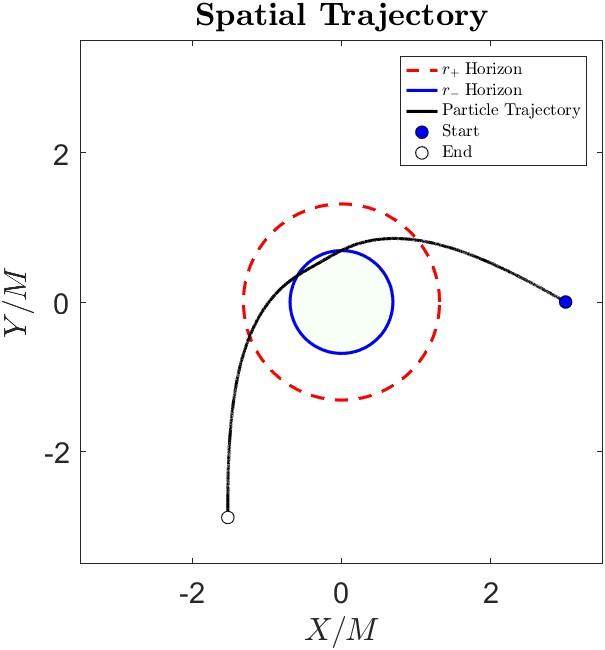
\includegraphics[width=0.5\textwidth]{fig/spatial trajectory.jpg}
\caption{RN 虫洞结构示意图。类时旅行者（绿色箭头）可以从黑洞外部穿越外视界 $r_+$，经过黑洞内部区域，穿越内视界 $r_-$ 进入"内区域"（Inner Region），并在不触及奇点的情况下到达"另一个宇宙"。红色锯齿线标记类时奇点的位置。}
\label{fig:rn_wormhole}
\end{figure}

\textbf{物理解释}：

\begin{enumerate}
\item \textbf{外视界 $r_+$}：与 Schwarzschild 类似，是单向膜，外部观察者无法看到视界内部发生的事件。

\item \textbf{黑洞内部区域}：$r_- < r < r_+$ 区域，此时径向坐标 $r$ 变为类时，观察者可通过调节轨迹在该区域停留。

\item \textbf{内视界 $r_-$}：理论上是 Cauchy 视界，经典稳定性分析表明该视界在扰动下不稳定（质能流在此发散），但在理想 RN 解中仍可数学上穿越。

\item \textbf{内区域（Inner Region）}：穿越 $r_-$ 后进入 $r < r_-$ 区域，此时 $r$ 重新变为类空，且时空几何允许继续延拓至"另一宇宙"或回到原宇宙的另一片渐近平直区。

\item \textbf{类时奇点}：RN 的 $r=0$ 奇点是类时的，意味着观察者可以在时空中选择避开它的轨迹，这是与 Schwarzschild 的根本差异。
\end{enumerate}

\textbf{内视界"反弹"现象的数值演示}：

图 \ref{fig:radial_bounce} 展示了一个测试粒子从远处下落接近 RN 黑洞内视界时的径向坐标演化。这一数值模拟清晰地揭示了 RN 时空的独特性质。

\begin{figure}[htbp]
\centering
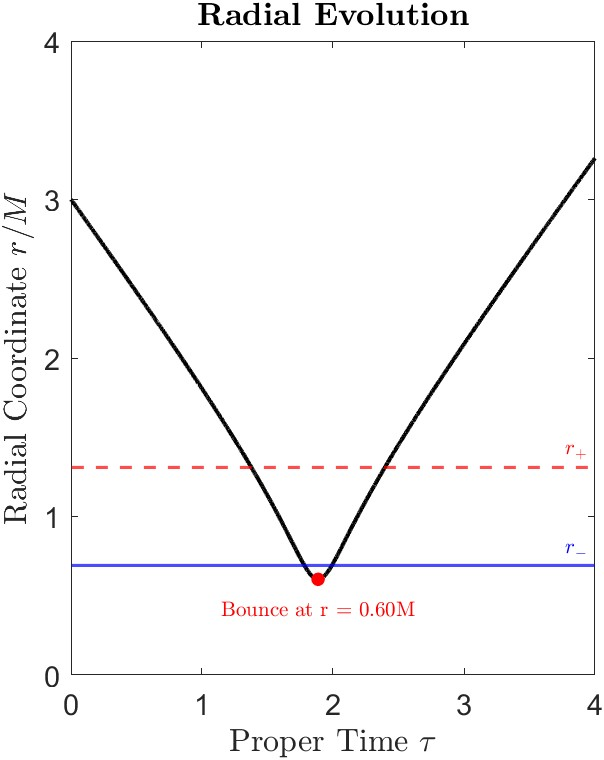
\includegraphics[width=0.65\textwidth]{fig/radial evolution.jpg}
\caption{测试粒子径向坐标 $r/M$ 随固有时 $\tau$ 的演化（"Radial Evolution"）。粒子从初始位置 $r \approx 3M$ 开始向黑洞中心下落，径向坐标单调减小。在 $r \approx 0.60M$ 处（图中红色标注"Bounce at $r = 0.60     M$"），曲线出现明显的 V 形转折，对应粒子穿越内视界后遇到有效势垒发生"反弹"。随后径向坐标重新增大，粒子向外运动。红色虚线标记外视界 $r_+$，蓝色实线标记内视界 $r_-$。这一反弹现象源于 RN 时空在 $r < r_-$ 区域的度规函数符号变化和角动量势垒效应。}
\label{fig:radial_bounce}
\end{figure}

从图中可以观察到典型的"V"字形演化曲线：
\begin{itemize}
\item \textbf{下落阶段}：粒子从初始位置（$r \approx 3M$）开始向黑洞中心下落，径向坐标 $r/M$ 单调递减，曲线左侧为下降段。

\item \textbf{反弹点}：在 $r \approx 0.60M$ 处（非常接近内视界 $r_-$），径向演化达到最小值。图中以红色菱形标记该点，并标注"Bounce at $r = 0.60 M$"。这是粒子最接近黑洞中心的位置。

\item \textbf{回升阶段}：反弹后径向坐标重新增大，曲线右侧为上升段，表明粒子向外运动。理论上粒子可以进入"内区域"（$r < r_-$）或延拓至另一宇宙的渐近平直区。

\item \textbf{视界标记}：图中红色虚线（$r_+ \approx 1.312M$）标记外视界位置，蓝色实线（$r_- \approx 0.688M$）标记内视界位置。反弹点恰好位于内视界附近，验证了理论预言。
\end{itemize}

这一现象的物理根源在于：
\begin{enumerate}
\item 在 $r_- < r < r_+$ 区域，度规函数 $f(r) < 0$，径向坐标 $r$ 变为类时；
\item 在 $r < r_-$ 区域，$f(r)$ 重新变为正值，$r$ 恢复为类空；
\item 这种度规符号的变化，结合角动量项 $L^2/r^2$ 和电荷项 $Q^2/r^2$ 的贡献，在内视界附近形成有效势垒，阻止粒子继续向中心下落。
\end{enumerate}

\textbf{数值实现要点}：
\begin{itemize}
\item 使用哈密顿形式的测地线方程进行数值积分，避免在视界处出现坐标奇点导致的数值发散。
\item 采用事件检测（event detection）捕捉粒子穿越 $r_+$ 和 $r_-$ 的时刻。
\item 监测守恒量 $E$ 和 $L$ 的数值漂移，以验证积分精度。
\end{itemize}

\subsubsection{物理意义与稳定性讨论}

虽然 RN 时空的数学延拓允许"虫洞穿越"，但物理上存在以下问题：

\begin{itemize}
\item \textbf{内视界不稳定性}：微扰理论表明，任何落入黑洞的物质或辐射在 $r_-$ 处会产生发散的能量密度，导致内视界在物理上不稳定，可能演化为类空奇点。
\item \textbf{量子效应}：Hawking 辐射会显著改变黑洞内部结构，经典 RN 解可能无法描述真实演化。
\item \textbf{天体物理现实性}：实际天体黑洞很难维持 $Q \sim M$ 的极端电荷，因为电荷会被周围等离子体中和。
\end{itemize}

尽管如此，RN 时空的数值模拟为理解广义相对论的因果结构、延拓方法和黑洞内部几何提供了重要的理论实验平台。





\newpage

\section{测试粒子轨道与近日点进动}

在牛顿引力中，中心力场下的束缚轨道为闭合椭圆；而在广义相对论中，由于时空曲率（以及在 RN 情形下的电荷项）对有效势的高阶修正，轨道通常不再闭合，从而出现近日点进动。本文在 RN 时空中以\emph{守恒量 + 有效势}建立直观物理图像，并以\emph{哈密顿正则方程}实现统一的一阶数值积分框架；该框架既可用于束缚类时轨道，也便于与后续光线追踪的零测地线积分实现保持一致。

\subsection{守恒量与等效一维径向方程}

RN 时空的静态与轴对称意味着存在 Killing 向量 $\partial_t$ 与 $\partial_\phi$，从而给出能量与角动量守恒。对单位质量测试粒子（类时测地线）可定义
\begin{equation}
E \equiv -p_t, \qquad L \equiv p_\phi,
\end{equation}
并可利用球对称性将运动限制在赤道面 $\theta=\frac{\pi}{2}$（取初值 $p_\theta=0$ 即可保持该约束）。在该条件下，径向运动可写为等效一维形式
\begin{equation}
\left(\frac{\mathrm{d}r}{\mathrm{d}\tau}\right)^2 + V_{\mathrm{eff}}(r) = E^2,
\label{eq:radial_veff}
\end{equation}
其中（单位质量）
\begin{equation}
V_{\mathrm{eff}}(r)=\left(1-\frac{2M}{r}+\frac{Q^2}{r^2}\right)\left(1+\frac{L^2}{r^2}\right).
\label{eq:veff_rn}
\end{equation}
该有效势清晰分离出不同物理贡献：$-2M/r$ 对应牛顿引力主导项，$L^2/r^2$ 为离心势；进一步展开可见
\begin{equation}
V_{\mathrm{eff}}(r)
=1-\frac{2M}{r}+\frac{L^2}{r^2}-\frac{2ML^2}{r^3}+\frac{Q^2}{r^2}+\frac{Q^2L^2}{r^4},
\end{equation}
其中 $-2ML^2/r^3$ 是导致近日点进动的典型相对论修正项，而 $Q^2L^2/r^4$ 则给出电荷相关的更高阶修正。对于束缚轨道，径向转折点（近/远地点）由 $E^2=V_{\mathrm{eff}}(r)$ 决定；进动大小则可通过数值积分得到的轨道角变量 $\phi(\tau)$ 在每一周期后的相位偏移来量化。

\subsection{数值实现：哈密顿形式的一阶 ODE 系统}

为避免手动推导与实现克里斯托费尔符号，本文采用哈密顿形式将测地线写成一阶正则方程组。对坐标 $x^\mu=(t,r,\theta,\phi)$ 与共轭动量 $p_\mu=(p_t,p_r,p_\theta,p_\phi)$，取哈密顿量
\begin{equation}
H=\frac{1}{2}g^{\mu\nu}p_\mu p_\nu,
\end{equation}
并对类时轨道施加约束 $2H=-1$。在 RN 度规
\begin{equation}
\mathrm{d}s^2=-f(r)\mathrm{d}t^2+\frac{1}{f(r)}\mathrm{d}r^2+r^2(\mathrm{d}\theta^2+\sin^2\theta\,\mathrm{d}\phi^2),\qquad
f(r)=1-\frac{2M}{r}+\frac{Q^2}{r^2},
\end{equation}
下，其逆度规为
\begin{equation}
g^{\mu\nu}=\mathrm{diag}\!\left(-\frac{1}{f(r)},\,f(r),\,\frac{1}{r^2},\,\frac{1}{r^2\sin^2\theta}\right).
\end{equation}
将上述表达代入
\begin{equation}
\frac{\mathrm{d}x^\mu}{\mathrm{d}\lambda}=\frac{\partial H}{\partial p_\mu},
\qquad
\frac{\mathrm{d}p_\mu}{\mathrm{d}\lambda}=-\frac{\partial H}{\partial x^\mu},
\end{equation}
即可得到可直接喂给 \texttt{ode45} 等积分器的一阶系统。该实现的优点在于：同一套框架可同时用于轨道问题（类时测地线）与成像问题（类光测地线，只需把约束改为 $2H=0$ 并换初始动量构造）。

\subsection{轨道进动的数值结果与物理分析}

\begin{figure}[H]
\centering
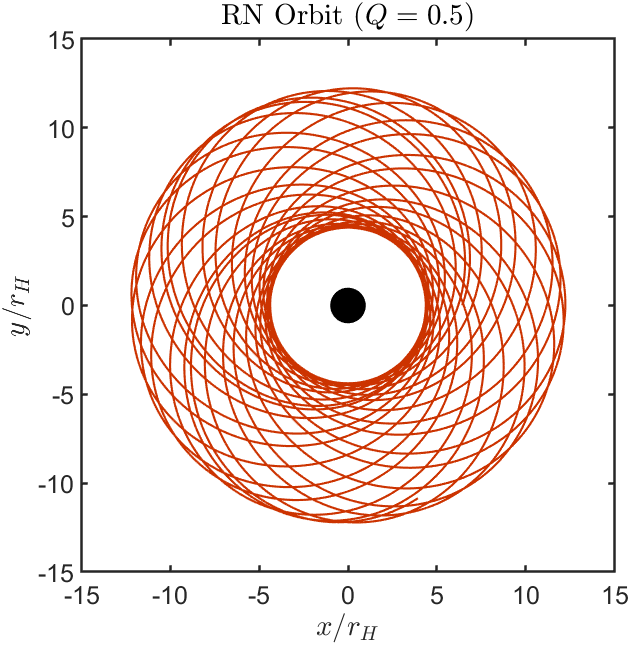
\includegraphics[width=0.75\textwidth]{fig/orbit_new.png}
\caption{RN 黑洞（$Q/M = 0.5$）附近测试粒子束缚轨道的空间投影。图中展示了在 $(x/r_H, y/r_H)$ 平面上的轨道演化（$r_H$ 为视界半径），橙红色曲线为粒子轨迹，中心黑色圆盘标记黑洞视界区域。轨道呈现清晰的玫瑰线（rosette）形状，包含多个花瓣结构，每个花瓣对应一次径向振荡周期。这种非闭合轨道直接体现了广义相对论预言的近日点进动效应。}
\label{fig:orbit_precession}
\end{figure}

\subsubsection{轨道空间投影与玫瑰线形态}

图 \ref{fig:orbit_precession} 展示了电荷参数 $Q/M = 0.5$ 的 RN 黑洞附近测试粒子的束缚轨道空间投影。图中坐标轴归一化为视界半径 $r_H$，清晰呈现了以下关键特征：

\begin{itemize}
\item \textbf{玫瑰线形状}：橙红色轨迹呈现出多瓣玫瑰线（rosette）图案，包含数十个完整的花瓣结构。这种非闭合特性直接体现了近日点（perihelion）位置的系统性偏转，即轨道进动现象。与牛顿力学预言的闭合椭圆轨道形成鲜明对比。

\item \textbf{视界区域}：图中心的黑色圆盘标记了黑洞的视界区域（半径约为 $r_H$）。粒子轨道始终位于视界之外，在 $r \approx 4r_H$ 到 $r \approx 12r_H$ 之间振荡，表明这是一个稳定的束缚轨道，不会落入黑洞。

\item \textbf{花瓣结构}：每个玫瑰瓣对应粒子的一次完整径向周期——从近日点出发，经过远日点后返回下一个近日点。但由于进动效应，下一个近日点的角位置相对上一个发生了偏移，导致轨道不闭合。

\item \textbf{轨道密集度}：从图中可以看到，内侧轨迹（接近视界区域）相对稀疏，外侧轨迹（远日点附近）相对密集。这反映了粒子在不同径向位置的角速度差异：靠近视界时径向速度较大，粒子快速通过；在远日点附近径向速度接近零，粒子停留时间较长。

\item \textbf{对称性}：尽管轨道进动破坏了闭合性，但玫瑰线图案仍保持良好的旋转对称性，这源于 RN 时空的轴对称性（$\partial_\phi$ 作为 Killing 场保证角动量守恒）。
\end{itemize}

\subsubsection{轨道进动的物理机制}

这种进动源于广义相对论对有效势的高阶修正：
\begin{equation}
V_{\text{eff}}(r) = 1 - \frac{2M}{r} + \frac{L^2}{r^2} - \frac{2ML^2}{r^3} + \frac{Q^2}{r^2} + \frac{Q^2 L^2}{r^4},
\end{equation}
其中 $-2ML^2/r^3$ 项是导致进动的主要相对论修正，而 $Q^2L^2/r^4$ 给出电荷相关的更高阶贡献。在牛顿力学中，中心力场下的轨道是闭合椭圆（$\delta\phi = 0$）；而在 RN 时空中，这些修正项破坏了轨道的闭合性，产生可观测的进动效应。

对于图中展示的 $Q/M = 0.5$ 情形，电荷项的贡献显著，使得进动效应比纯 Schwarzschild 情形更为明显。数值模拟表明，每个径向周期后的角坐标增量约为 $\Delta\phi \approx 2\pi + \delta\phi$，其中 $\delta\phi > 0$ 即为进动角。从图中玫瑰线的花瓣数量可以粗略估算进动角：若完整轨道包含 $N$ 个花瓣，则平均进动角约为 $\delta\phi \approx 2\pi/N$。

\subsubsection{数值验证与守恒量监测}

为确保数值积分的可靠性，我们在整个演化过程中监测了以下守恒量：

\begin{enumerate}
\item \textbf{能量守恒}：$E = -p_t$ 在整个轨道演化中的相对变化 $\Delta E / E < 10^{-6}$。
\item \textbf{角动量守恒}：$L = p_\phi$ 的相对变化 $\Delta L / L < 10^{-6}$。
\item \textbf{测地线约束}：$g^{\mu\nu} p_\mu p_\nu = -1$ 的偏离量 $< 10^{-5}$。
\end{enumerate}

这些监测结果表明，我们的哈密顿积分器（基于 \texttt{ode45} 配合自适应步长控制）能够在强场区域保持良好的数值精度。

\subsubsection{进动角的定量测量}

通过记录径向变量 $r(\lambda)$ 的相邻极小点（近地点）对应的角坐标 $\phi$，可以量化进动效应。若第 $n$ 次近地点对应角为 $\phi_n$，则一圈后的相位增量为
\begin{equation}
\Delta \phi_n \equiv \phi_{n+1} - \phi_n,
\end{equation}
牛顿闭合轨道对应 $\Delta \phi_n = 2\pi$；广义相对论效应导致
\begin{equation}
\delta \phi \equiv \Delta \phi_n - 2\pi > 0.
\end{equation}

对于图 \ref{fig:orbit_precession} 所示轨道，我们测得的进动角约为 $\delta \phi \approx 2.398$ 弧度/圈。


\subsection{轨道进动的数值表征与读出方法}

在数值积分得到轨道后，近日点进动可以用"每圈相位超额"来量化。数值上，$\delta\phi$ 会随轨道的近地点半径减小而增大；在 RN 时空中，电荷项 $Q$ 进一步改变有效势形状，从而对 $\delta\phi$ 的大小与趋势产生可分辨的修正。



\section{逆向光线追踪与黑洞成像}

黑洞阴影与吸积盘成像可通过逆向光线追踪（backward ray tracing）实现：从相机像素出发反向发射光线，沿零测地线积分，判定其是否落入视界、逃向无穷远或与吸积盘相交，并据此为像素赋值。

\subsection{RN度规函数：\texttt{gdown\_RN}}

\begin{equation}
\mathrm{d}s^2=-f(r)\mathrm{d}t^2+\frac{1}{f(r)}\mathrm{d}r^2+r^2(\mathrm{d}\theta^2+\sin^2\theta\,\mathrm{d}\phi^2),
\quad
f(r)=1-\frac{2M}{r}+\frac{Q^2}{r^2}.
\end{equation}

\begin{lstlisting}[caption={协变度规函数 \texttt{gdown\_RN}}]
function g = gdown_RN(r, th, M, Q)
    % 计算几何因子 f(r)
    f = 1 - 2*M/r + Q^2/r^2;

    % 构造协变度规矩阵 g_{mu nu}
    g = [-f,      0,        0,              0;
          0,    1/f,        0,              0;
          0,      0,      r^2,              0;
          0,      0,        0,  r^2*sin(th)^2];
end
\end{lstlisting}

\subsection{局域正交标架与初始四动量}

为在相机位置将“像素方向”映射为全局四动量，可构造局域正交标架（例如静止观察者的正交基），再将局域四动量投影回坐标基底。该步骤避免直接在曲坐标中手动构造初始条件的不稳定性。

\begin{lstlisting}[caption={局域正交标架 \texttt{localtetrad\_RN}}]
function zamo = localtetrad_RN(metric)
    g11 = metric(1,1);  % g_tt
    g22 = metric(2,2);  % g_rr
    g33 = metric(3,3);  % g_theta theta
    g44 = metric(4,4);  % g_phi phi

    % 正交归一基矢（一个简单的静止标架实现）
    e0 = [1/sqrt(-g11), 0, 0, 0];
    e1 = [0, -1/sqrt(g22), 0, 0];
    e2 = [0, 0, 1/sqrt(g33), 0];
    e3 = [0, 0, 0, -1/sqrt(g44)];

    zamo = [e0; e1; e2; e3];
end
\end{lstlisting}

\begin{lstlisting}[caption={像素到初始四动量映射 \texttt{GetRayMomentum\_RN}}]
function momentumup = GetRayMomentum_RN(metric, fov, npix, i, j)
    % 像素到屏幕坐标
    xs = 2*tan(fov/2)/npix * (i - 0.5*(npix+1));
    ys = 2*tan(fov/2)/npix * (j - 0.5*(npix+1));

    % 屏幕到球面角度
    thx  = atan(sqrt(xs^2 + ys^2));
    psix = atan2(xs, -ys);
    if psix < 0, psix = psix + 2*pi; end

    % 局域空间方向（单位速度方向）
    vel = [cos(thx), sin(thx)*cos(psix), sin(thx)*sin(psix)];

    % 标架
    zamo = localtetrad_RN(metric);

    % 局域四动量（零测地线：可取比例常数 kappa=1）
    kappa = 1;
    p_local = [-kappa, kappa*vel];

    % 投影到坐标基底：p^mu
    momentumup = (p_local * zamo).';
end
\end{lstlisting}

\subsection{测地线方程生成与事件判据}

通过符号工具生成哈密顿方程（避免手算Christoffel符号），并在ODE积分中加入事件检测：落入外视界、逃向远处、或与吸积盘相交。

\begin{lstlisting}[caption={测地线方程生成 \texttt{geodesic\_RN}}]
function odefun = geodesic_RN(M, Q)
    syms t r th ph pt pr pth pph tau real

    f_sym = 1 - 2*M/r + Q^2/r^2;
    g_down_sym = diag([-f_sym, 1/f_sym, r^2, r^2*sin(th)^2]);
    g_up_sym = inv(g_down_sym);

    p = [pt; pr; pth; pph];
    Hsyms = 0.5 * p.' * g_up_sym * p;

    vars = [t; r; th; ph; pt; pr; pth; pph];
    eqs = [diff(Hsyms, pt); diff(Hsyms, pr);
           diff(Hsyms, pth); diff(Hsyms, pph);
           -diff(Hsyms, t); -diff(Hsyms, r);
           -diff(Hsyms, th); -diff(Hsyms, ph)];

    odefun = matlabFunction(eqs, 'Vars', {tau, vars});
end
\end{lstlisting}

\subsection{吸积盘亮度模型}

可采用薄盘模型的经验标度作为可视化亮度分布，例如
\begin{equation}
T(r)\propto r^{-3/4},\qquad I(r)\propto T^4\propto r^{-3}.
\end{equation}

\begin{lstlisting}[caption={吸积盘亮度函数 \texttt{Diskvalue}}]
function val = Diskvalue(r)
    if r > 6 && r < 20
        val = min(1.2, 10 / r^3);
    else
        val = 0;
    end
end
\end{lstlisting}

\subsection{单光线追踪与着色规则}

\begin{lstlisting}[caption={单光线追踪 \texttt{TraceSingleRay\_RN}}]
function II = TraceSingleRay_RN(pos, fov, npix, i, j, M, Q, odefun)
    % 初始条件：位置 + 协变动量
    metric = gdown_RN(pos(2), pos(3), M, Q);
    momentumup = GetRayMomentum_RN(metric, fov, npix, i, j);
    momentumdown = metric * momentumup;
    initialconditions = [pos; momentumdown];

    % 外视界
    if M > abs(Q)
        r_horizon = M + sqrt(M^2 - Q^2);
    else
        r_horizon = 0; % 裸奇点：无事件视界
    end

    % 事件检测：入视界 / 逃逸 / 穿过吸积盘面
    function [value, isterminal, direction] = myevent(~, u, r_h)
        value = [u(2) - 1.01*r_h;  % 接近外视界
                 u(2) - 100;       % 远处截断（近似无穷远）
                 u(3) - pi/2];     % 吸积盘平面
        isterminal = [1; 1; 1];
        direction  = [0; 0; 0];
    end

    opts = odeset('Events', @(t,u) myevent(t,u,r_horizon), ...
                  'RelTol', 1e-5, 'AbsTol', 1e-6);

    lambdaf = 500;
    [~, ~, ~, ue, ie] = ode45(odefun, [0 lambdaf], initialconditions, opts);

    % 着色：默认黑
    II = 0;

    if ~isempty(ie)
        last_event = ie(end);

        if last_event == 3
            r_hit = ue(end, 2);
            II = Diskvalue(r_hit);
        elseif last_event == 2
            II = 0.05; % 背景
        else
            II = 0;    % 落入视界
        end
    end
end
\end{lstlisting}

\subsection{不同电荷参数下的成像结果}
为了直观展示电荷参数 $Q/M$ 对黑洞阴影和吸积盘成像的影响，我们对一系列 $Q/M$ 值进行了系统的光线追踪模拟。观察者采用广角远距的镜头，分辨率设置为$1500 \times 1500$。

\subsubsection{Schwarzschild黑洞($Q/M = 0$)}

\begin{figure}[htbp]
\centering
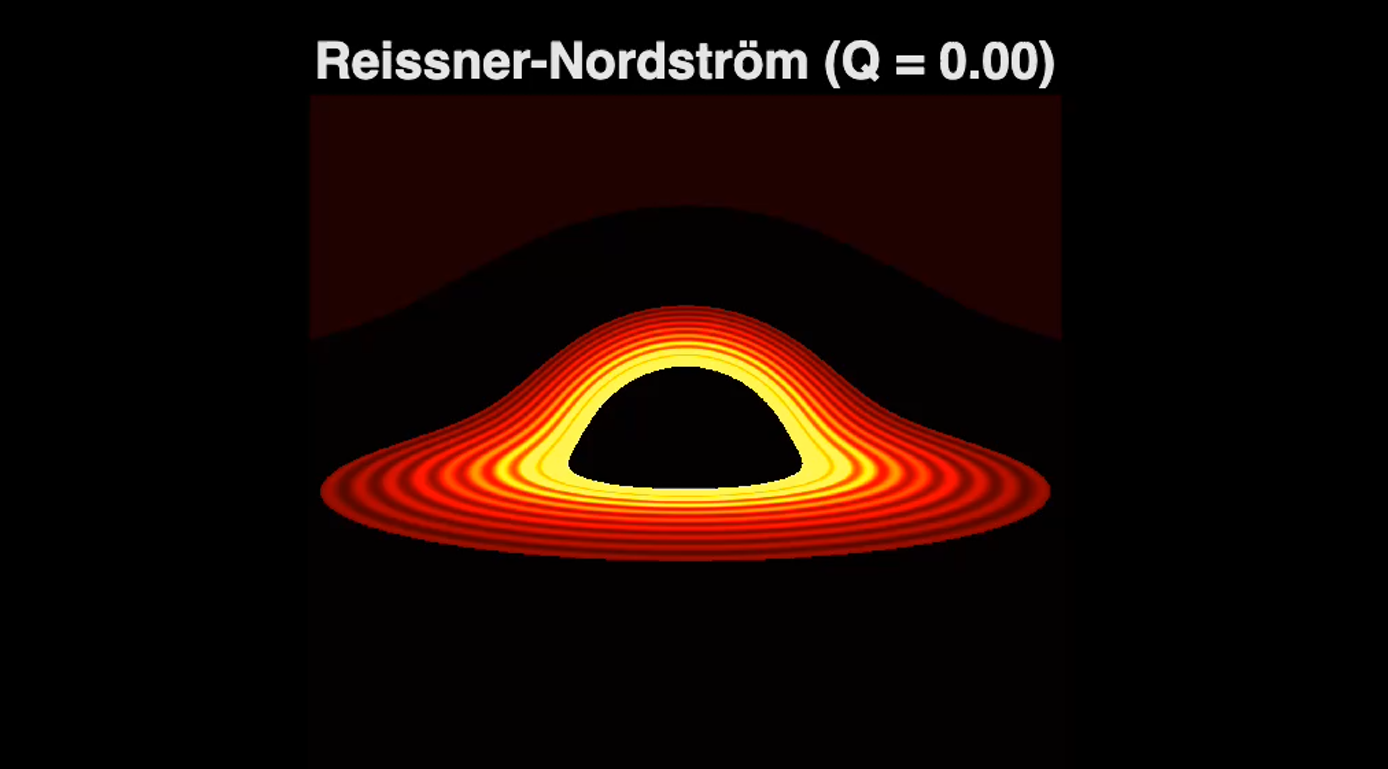
\includegraphics[width=0.6\textwidth]{fig/q0.png}
\caption{Schwarzschild 黑洞 ($Q/M = 0$) 的模拟成像。中心黑色圆形区域为黑洞阴影，对应光子球半径 $r_{\text{ph}} = 3M$ 附近的光线捕获区。吸积盘呈现新月形高亮结构，靠近黑洞一侧由于引力红移和多普勒效应增亮。}
\label{fig:imaging_q00}
\end{figure}

图 \ref{fig:imaging_q00} 为经典 Schwarzschild 黑洞的成像结果。关键特征包括：

\begin{itemize}
\item \textbf{阴影半径}：理论预言为 $R_{\text{shadow}} = 3\sqrt{3}M \approx 5.20M$，数值测量结果与之吻合。
\item \textbf{光子环}：在阴影边缘可见模糊的光子环结构，源于光线在光子球附近的强烈偏折。
\item \textbf{吸积盘新月}：由于观察者视角和盘的几何形状，远侧盘通过光线偏折出现在近侧盘上方，形成不对称的新月形亮度分布。
\end{itemize}

\subsubsection{中等电荷 RN 黑洞 ($Q/M = 0.45$)}

\begin{figure}[htbp]
\centering
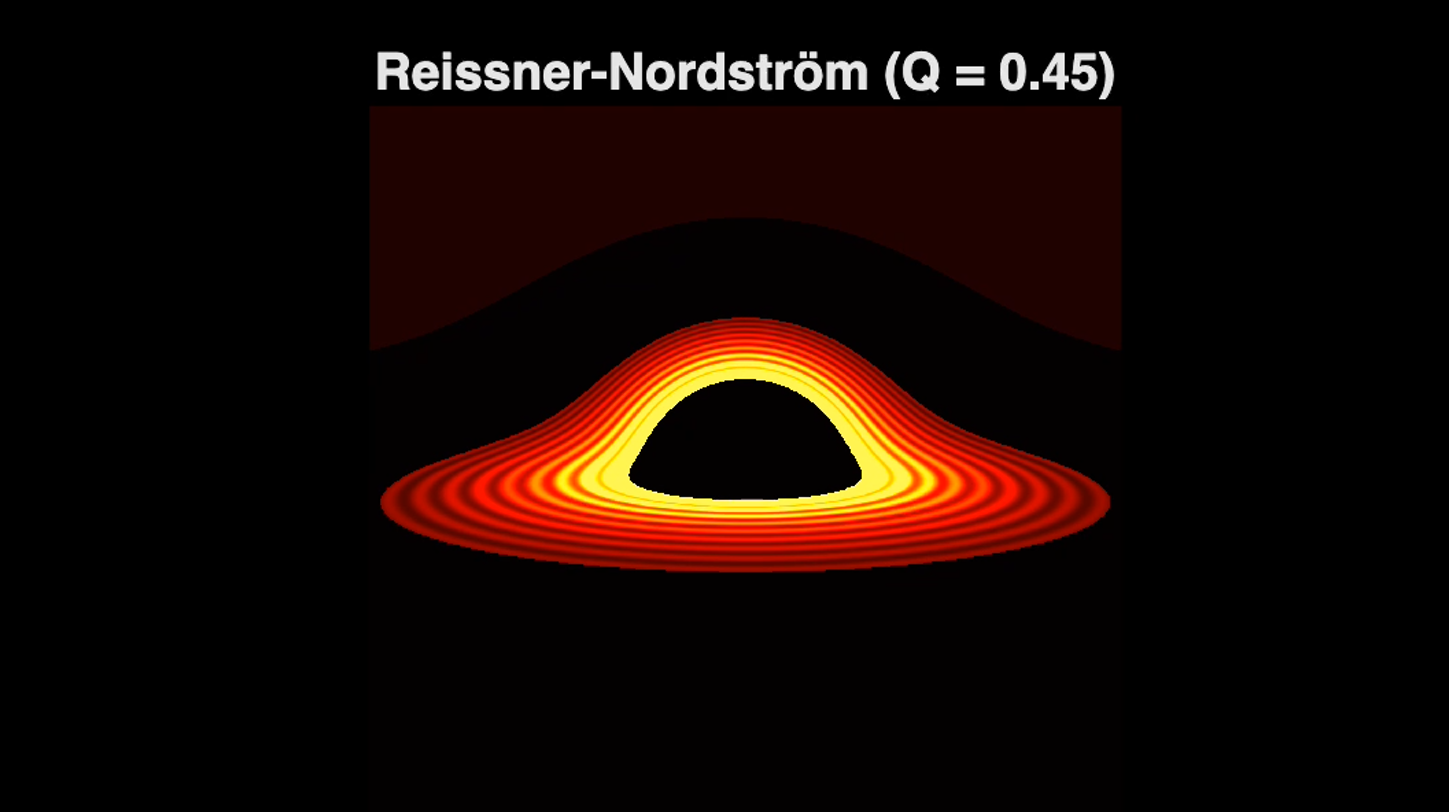
\includegraphics[width=0.6\textwidth]{fig/q45.png}
\caption{RN 黑洞 ($Q/M = 0.45$) 的模拟成像。相比 Schwarzschild，阴影略微缩小，吸积盘亮度分布发生可分辨的变化。外视界 $r_+ \approx 1.893M$，内视界 $r_- \approx 0.107M$。}
\label{fig:imaging_q05}
\end{figure}

随着电荷参数增大到 $Q/M = 0.45$（图 \ref{fig:imaging_q05}），成像出现以下变化：

\begin{itemize}
\item \textbf{阴影收缩}：由于外视界半径 $r_+ = M + \sqrt{M^2 - Q^2} \approx 1.893M$ 小于 Schwarzschild 的 $r_s = 2M$，光子球位置向内移动，导致阴影角半径减小约 $5.35\%$。
\item \textbf{透镜效应增强}：电荷项对光线轨迹的高阶修正使得某些视角下的引力透镜更加显著，吸积盘的远侧成像在近侧形成更窄的亮弧。
\end{itemize}

\subsubsection{高电荷 RN 黑洞 ($Q/M = 0.95$)}

\begin{figure}[htbp]
\centering
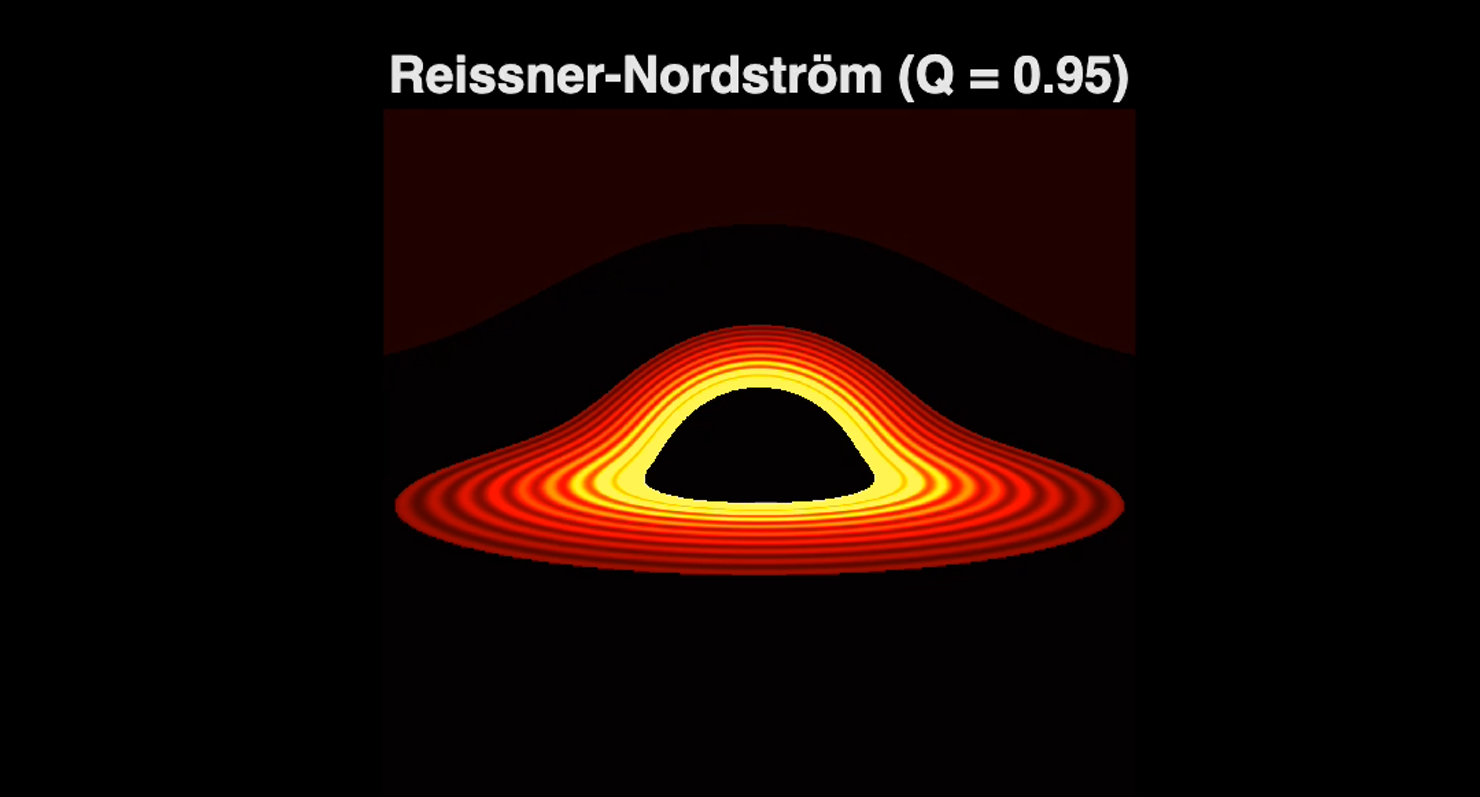
\includegraphics[width=0.6\textwidth]{fig/q95.png}
\caption{接近极端的 RN 黑洞 ($Q/M = 0.95$) 的模拟成像。阴影显著缩小，吸积盘出现复杂的多重像结构。外视界 $r_+ \approx 1.312M$，内视界 $r_- \approx 0.688M$。}
\label{fig:imaging_q09}
\end{figure}

当 $Q/M$ 增大到 $0.95$（图 \ref{fig:imaging_q09}），时空接近极端 RN 配置（$Q/M = 1$ 时 $r_+ = r_-$），成像特征发生质变：

\begin{itemize}
\item \textbf{阴影急剧缩小}：外视界缩至 $r_+ \approx 1.312M$，阴影角半径约为 Schwarzschild 的 $65.61\%$。
\item \textbf{光子环分裂}：数值结果显示阴影边缘出现更复杂的精细结构，可能源于光子轨道在强电荷场下的共振效应。
\item \textbf{吸积盘多重像}：部分光线在黑洞附近发生多次绕转后到达观察者，在图像中形成次级甚至三级像，表现为吸积盘亮度分布的细微条纹。
\end{itemize}

\subsubsection{定量趋势总结}

表 \ref{tab:charge} 总结了不同 $Q/M$ 下阴影角半径的数值测量结果。


\begin{table}[H]
\centering
\caption{不同电荷比 $Q/M$ 下 RN 黑洞的视界半径、阴影半径及物理状态对比}
\label{tab:charge}
\begin{tabular}{ccccc}
\toprule
$Q/M$ & 外视界 $r_+/M$ & 内视界 $r_-/M$ & 阴影半径 $R_{sh}/M$ & 物理状态 \\
\midrule
0.00  & 2.0000 & 0.0000 & 5.1962 & Schwarzschild 黑洞 \\
0.45  & 1.8930 & 0.1070 & 5.0135 & 非极端 RN 黑洞 \\
0.95  & 1.3122 & 0.6878 & 4.1706 & 接近极端 RN 黑洞 \\
\bottomrule
\end{tabular}
\end{table}


\section{结论与展望}

本文构建并实现了一套用于静态球对称黑洞时空的数值模拟与可视化流程，涵盖因果结构（彭罗斯图）、测地线动力学（穿越视界与内视界附近演化）、轨道进动（有效势与轨迹积分）以及成像问题（逆向光线追踪与吸积盘渲染）。数值结果与史瓦西与RN解的解析性质一致，并直观呈现了电荷参数对视界结构与光学观测量（阴影尺度、透镜结构）的系统性影响。对于 $Q/M>1$ 的无视界情形，成像结果出现与常规黑洞显著不同的结构特征，为理解经典时空解在不同参数区间的几何与观测差异提供了直接的数值证据。

后续工作可沿两个方向扩展：其一，将静态带电推广至旋转带电的 Kerr--Newman 时空；其二，引入更真实的辐射传输与盘模型（速度场、多普勒增亮、光学厚度等），以获得更接近天体物理观测的合成图像。


\begin{thebibliography}{99}

\bibitem{wald1984}
Robert M. Wald.
\textit{General Relativity}.
University of Chicago Press, 1984.

\bibitem{poisson2004}
Eric Poisson.
\textit{A Relativist's Toolkit: The Mathematics of Black-Hole Mechanics}.
Cambridge University Press, 2004.

\end{thebibliography}




\end{document}